\item {\bf Double Descent}

The following set of questions are going to discuss a phenomenon known as deep double descent. This is a modern research topic that is still not very well understood. Read the passage below and answer the related questions. For those interested in learning more, visit OpenAI’s blog post here: \url{https://openai.com/blog/deep-double-descent/}\\

When selecting a class of models for a machine learning problem, a classical statistician would caution that using a large class will result in high variance/overfitting. A more contemporary ML practitioner may suggest using larger and larger models based on empirical findings over the last ten years. Recent work has shown that neither of these methodologies uphold exactly. Among many kinds of deep learning models we observe a double descent phenomenon where as model size/complexity increases, test performance first improves, then gets worse as the model begins to overfit, and then continues to improve as we increase model size/complexity. This peak in test error occurs in a ‘critical regime’, where the model is large/complex enough to almost interpolate (perfectly fit) the training set. \\

Intuitively, as one increases the size of an under-parameterized model that is unable to perfectly fit the training data, there is one specific weight configuration that best fits the data. Thus in the complexity regime where the model can approximately interpolate the training data, there is one weight configuration that results in this approximate interpolation. This weight configuration is unlikely to generalize to test data, hence the peak in test error. Once we enter the over-parameterized region there are many models which can perfectly fit the training data. For reasons we don’t yet understand, the implicit bias of stochastic gradient descent (SGD) leads us to find models which both interpolate the training data and generalize well. Note that the implicit bias of SGD refers to the tendency over-parameterized models which are trained using SGD to generalize well to unseen data. \\

We also note a model size regime where having more training data hurts the performance of the model. This is illustrated in the plot below
\begin{center}
    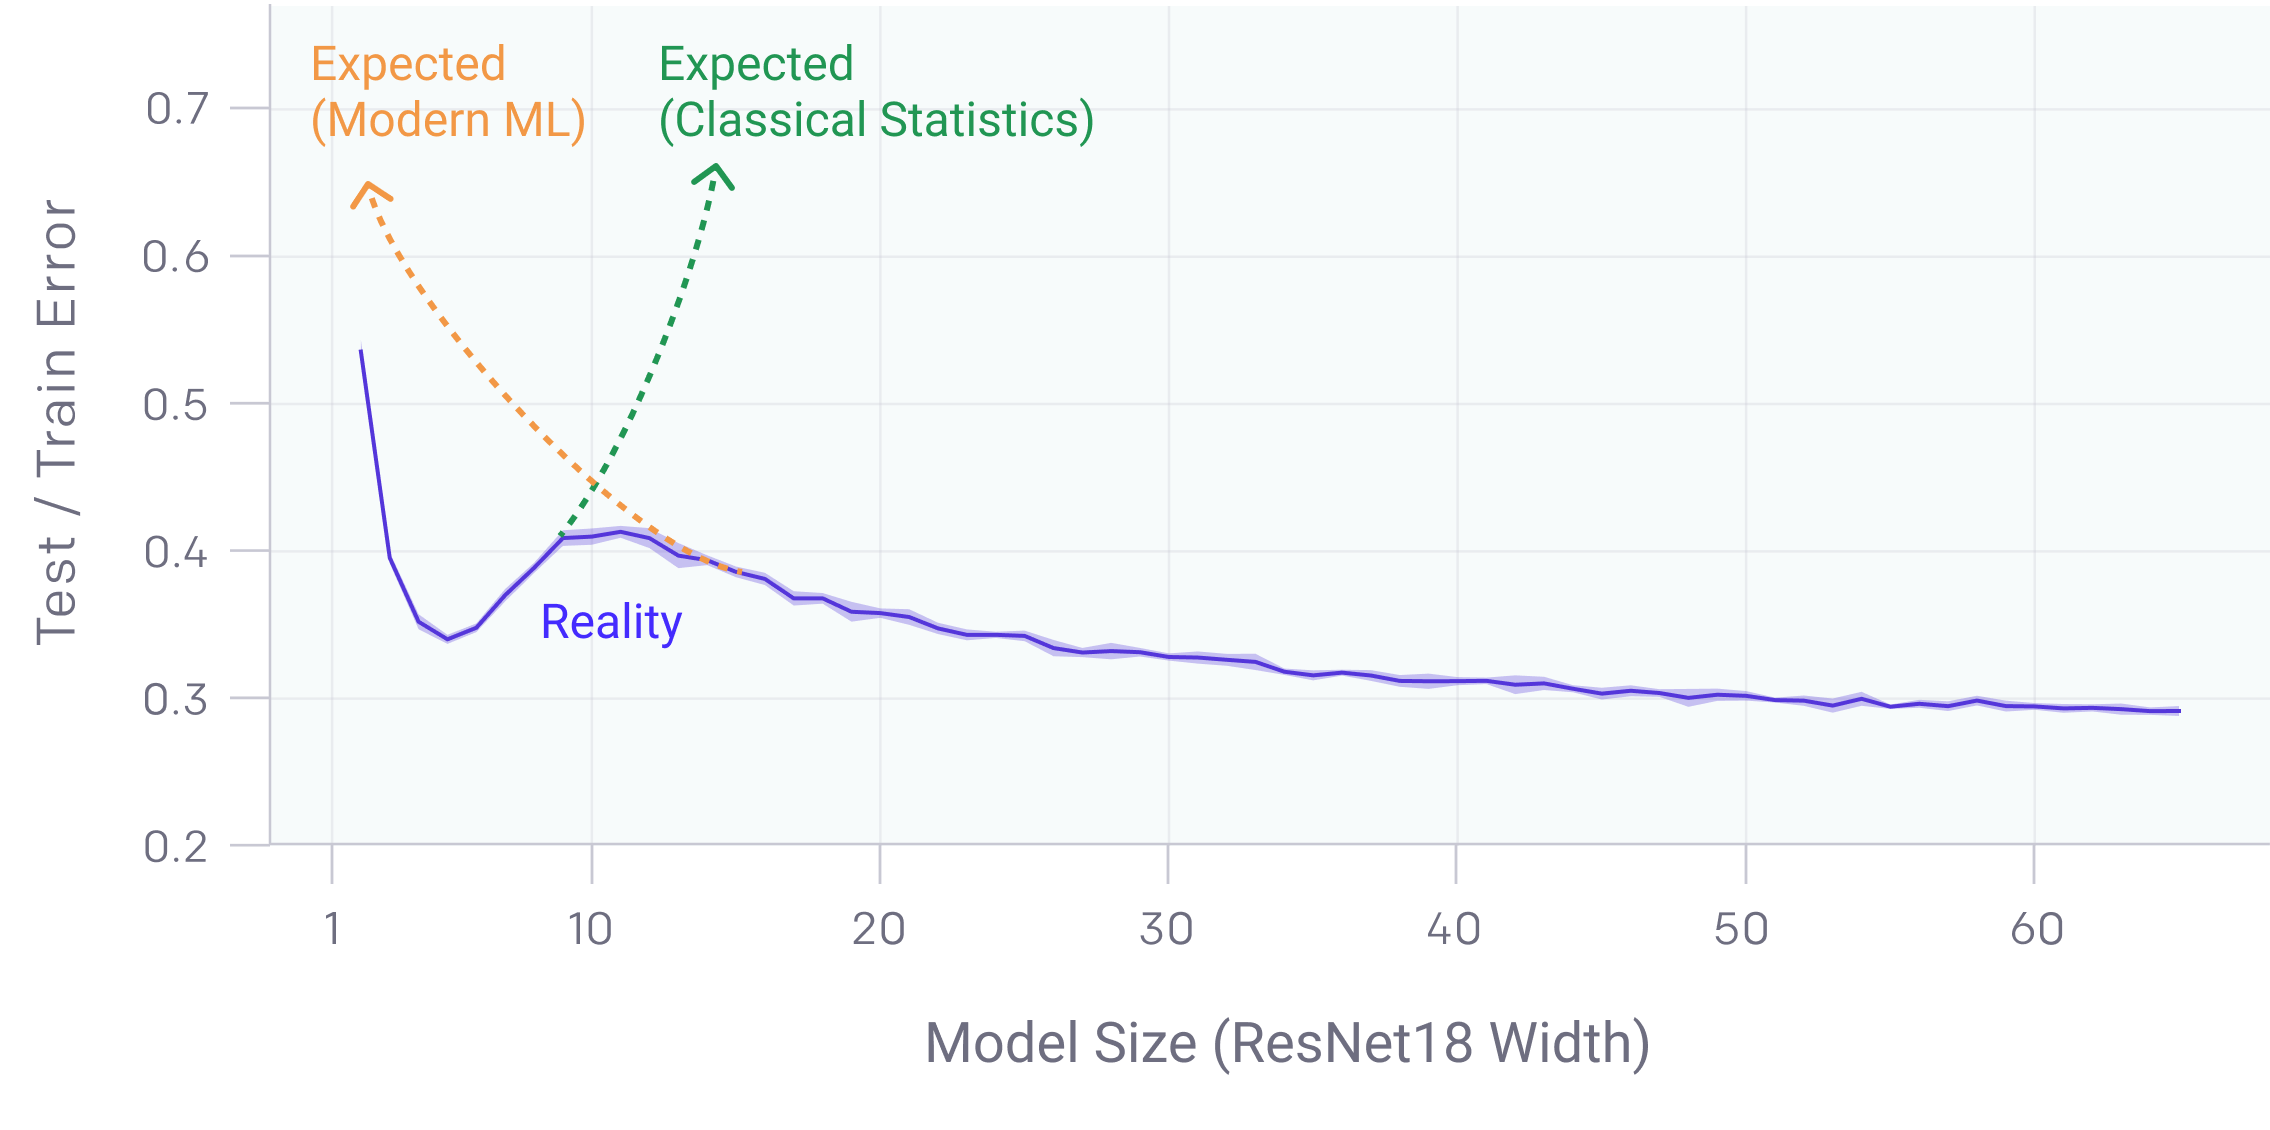
\includegraphics[scale=0.3]{double-descent/dd.png}
\end{center}

Lastly, we note a phenomenon dubbed epoch-wise double descent, where the test error decreases with additional training, then increases as the training data is almost perfectly fit, and then continues to decrease. This is shown in the plot below:
\begin{center}
    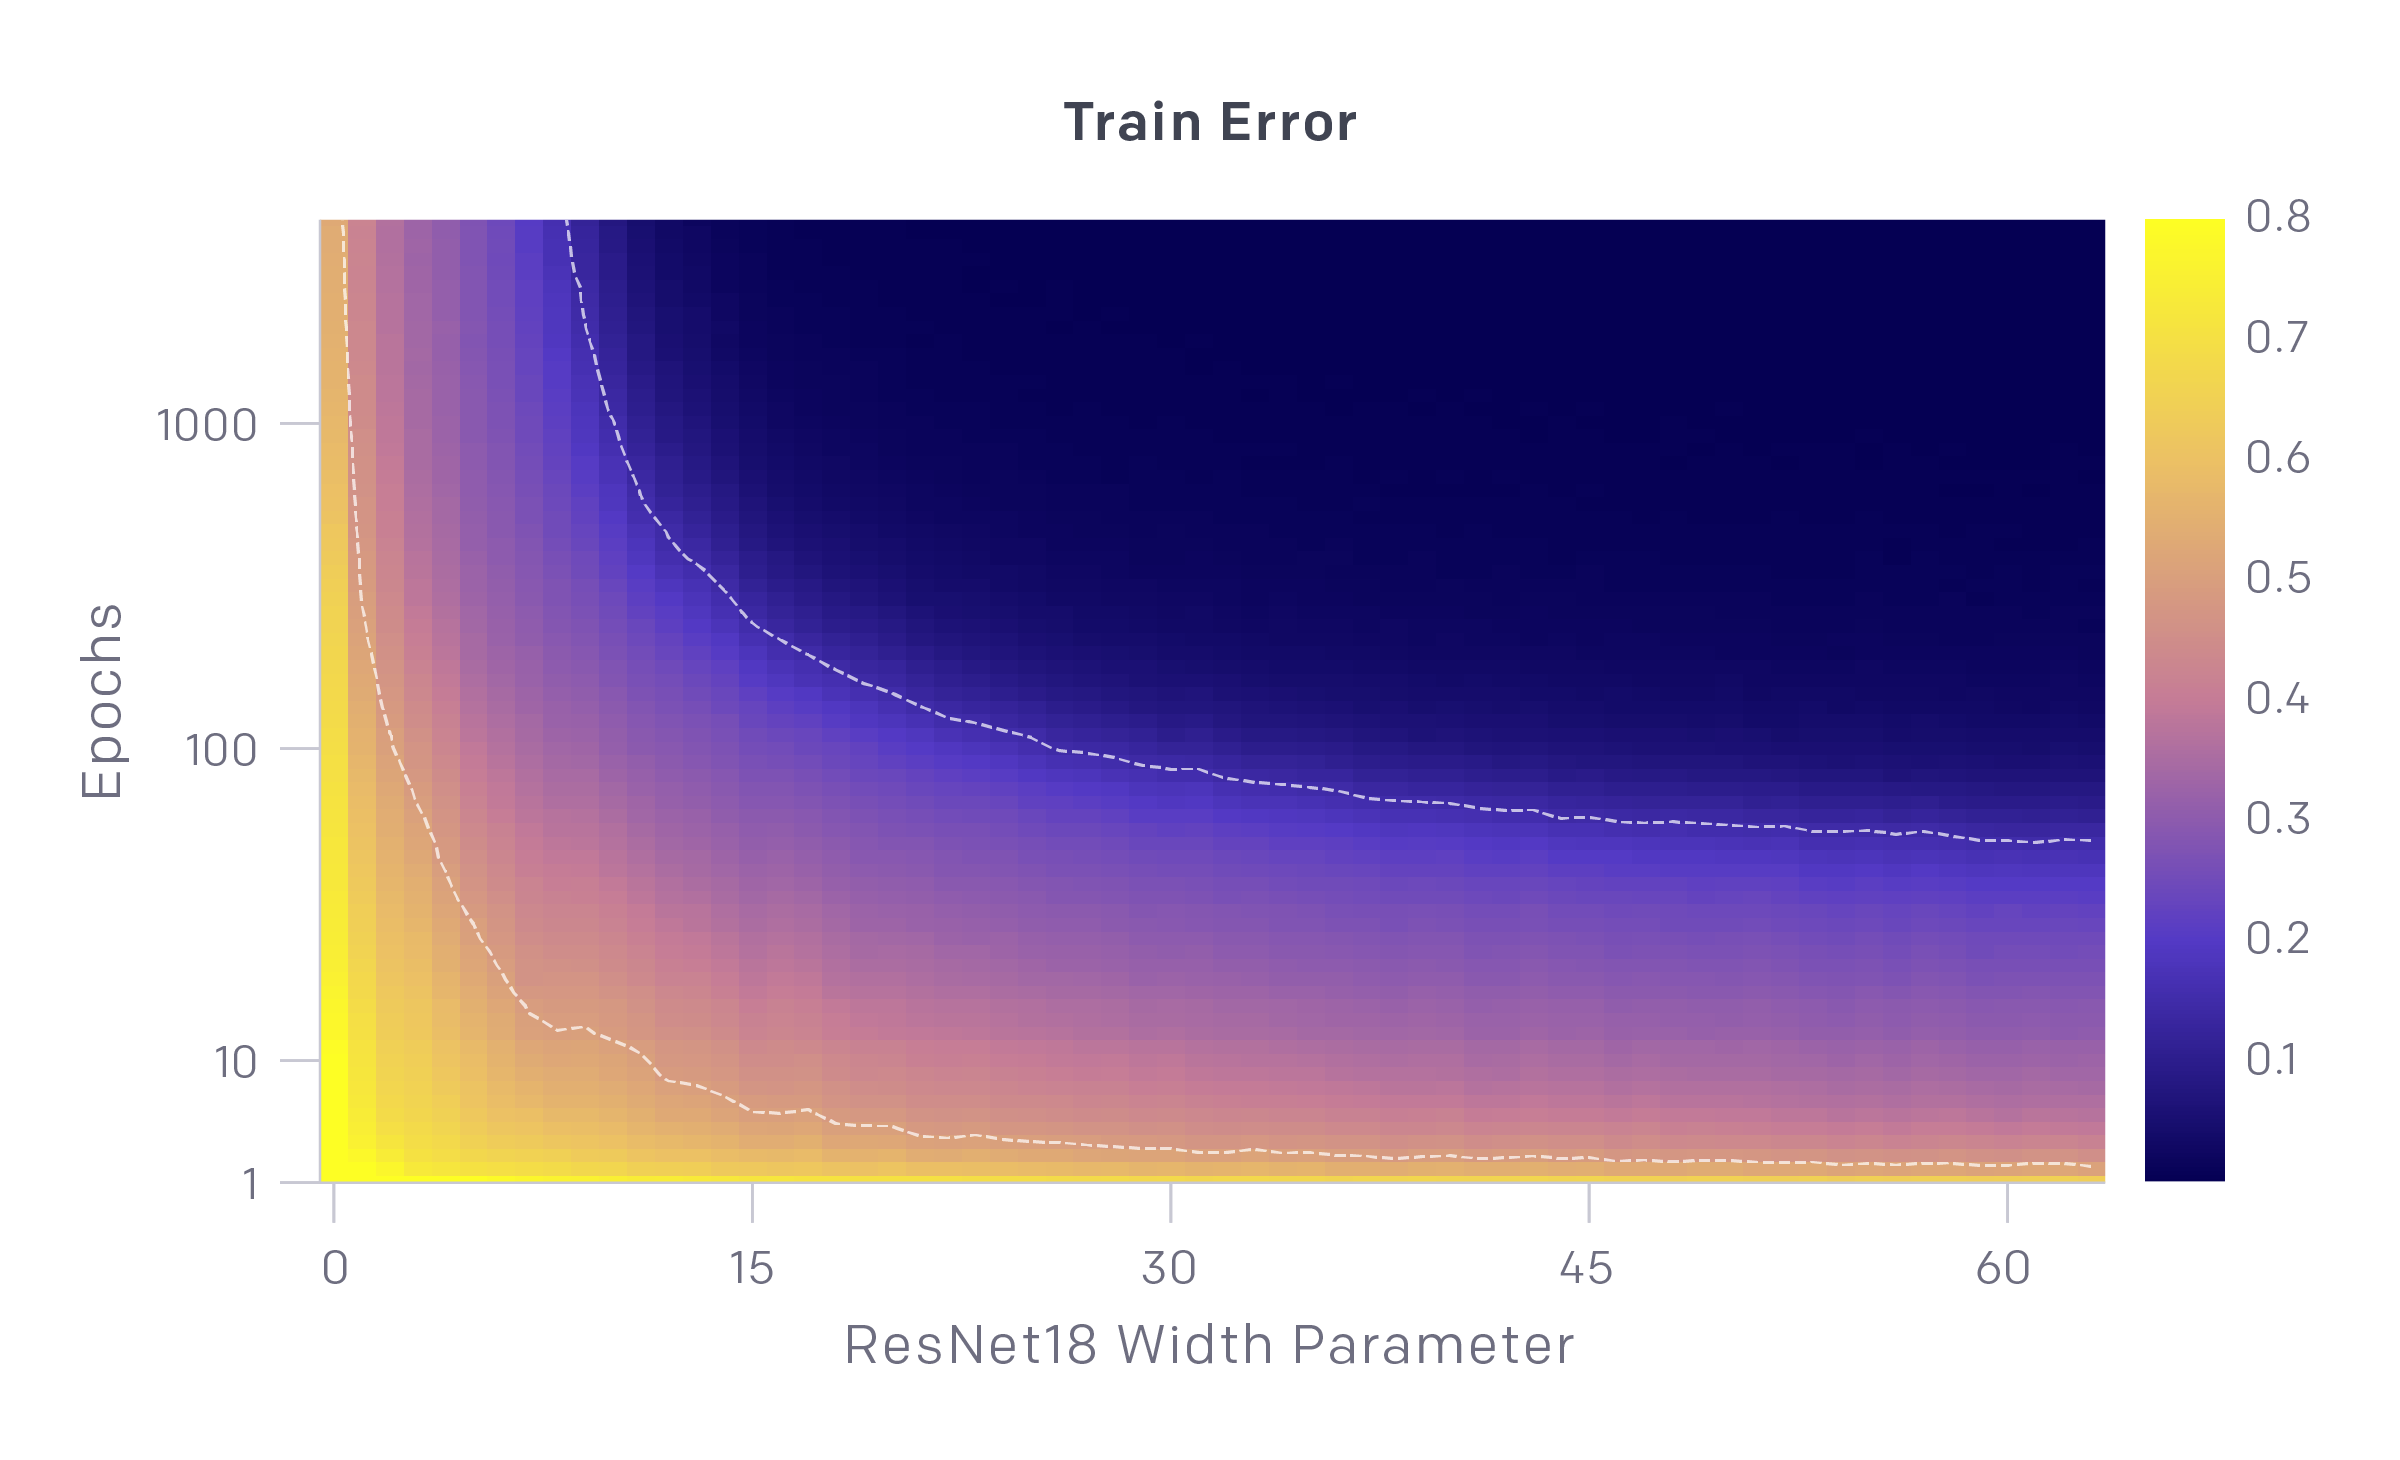
\includegraphics[scale=0.1]{double-descent/epoch_train.png}
    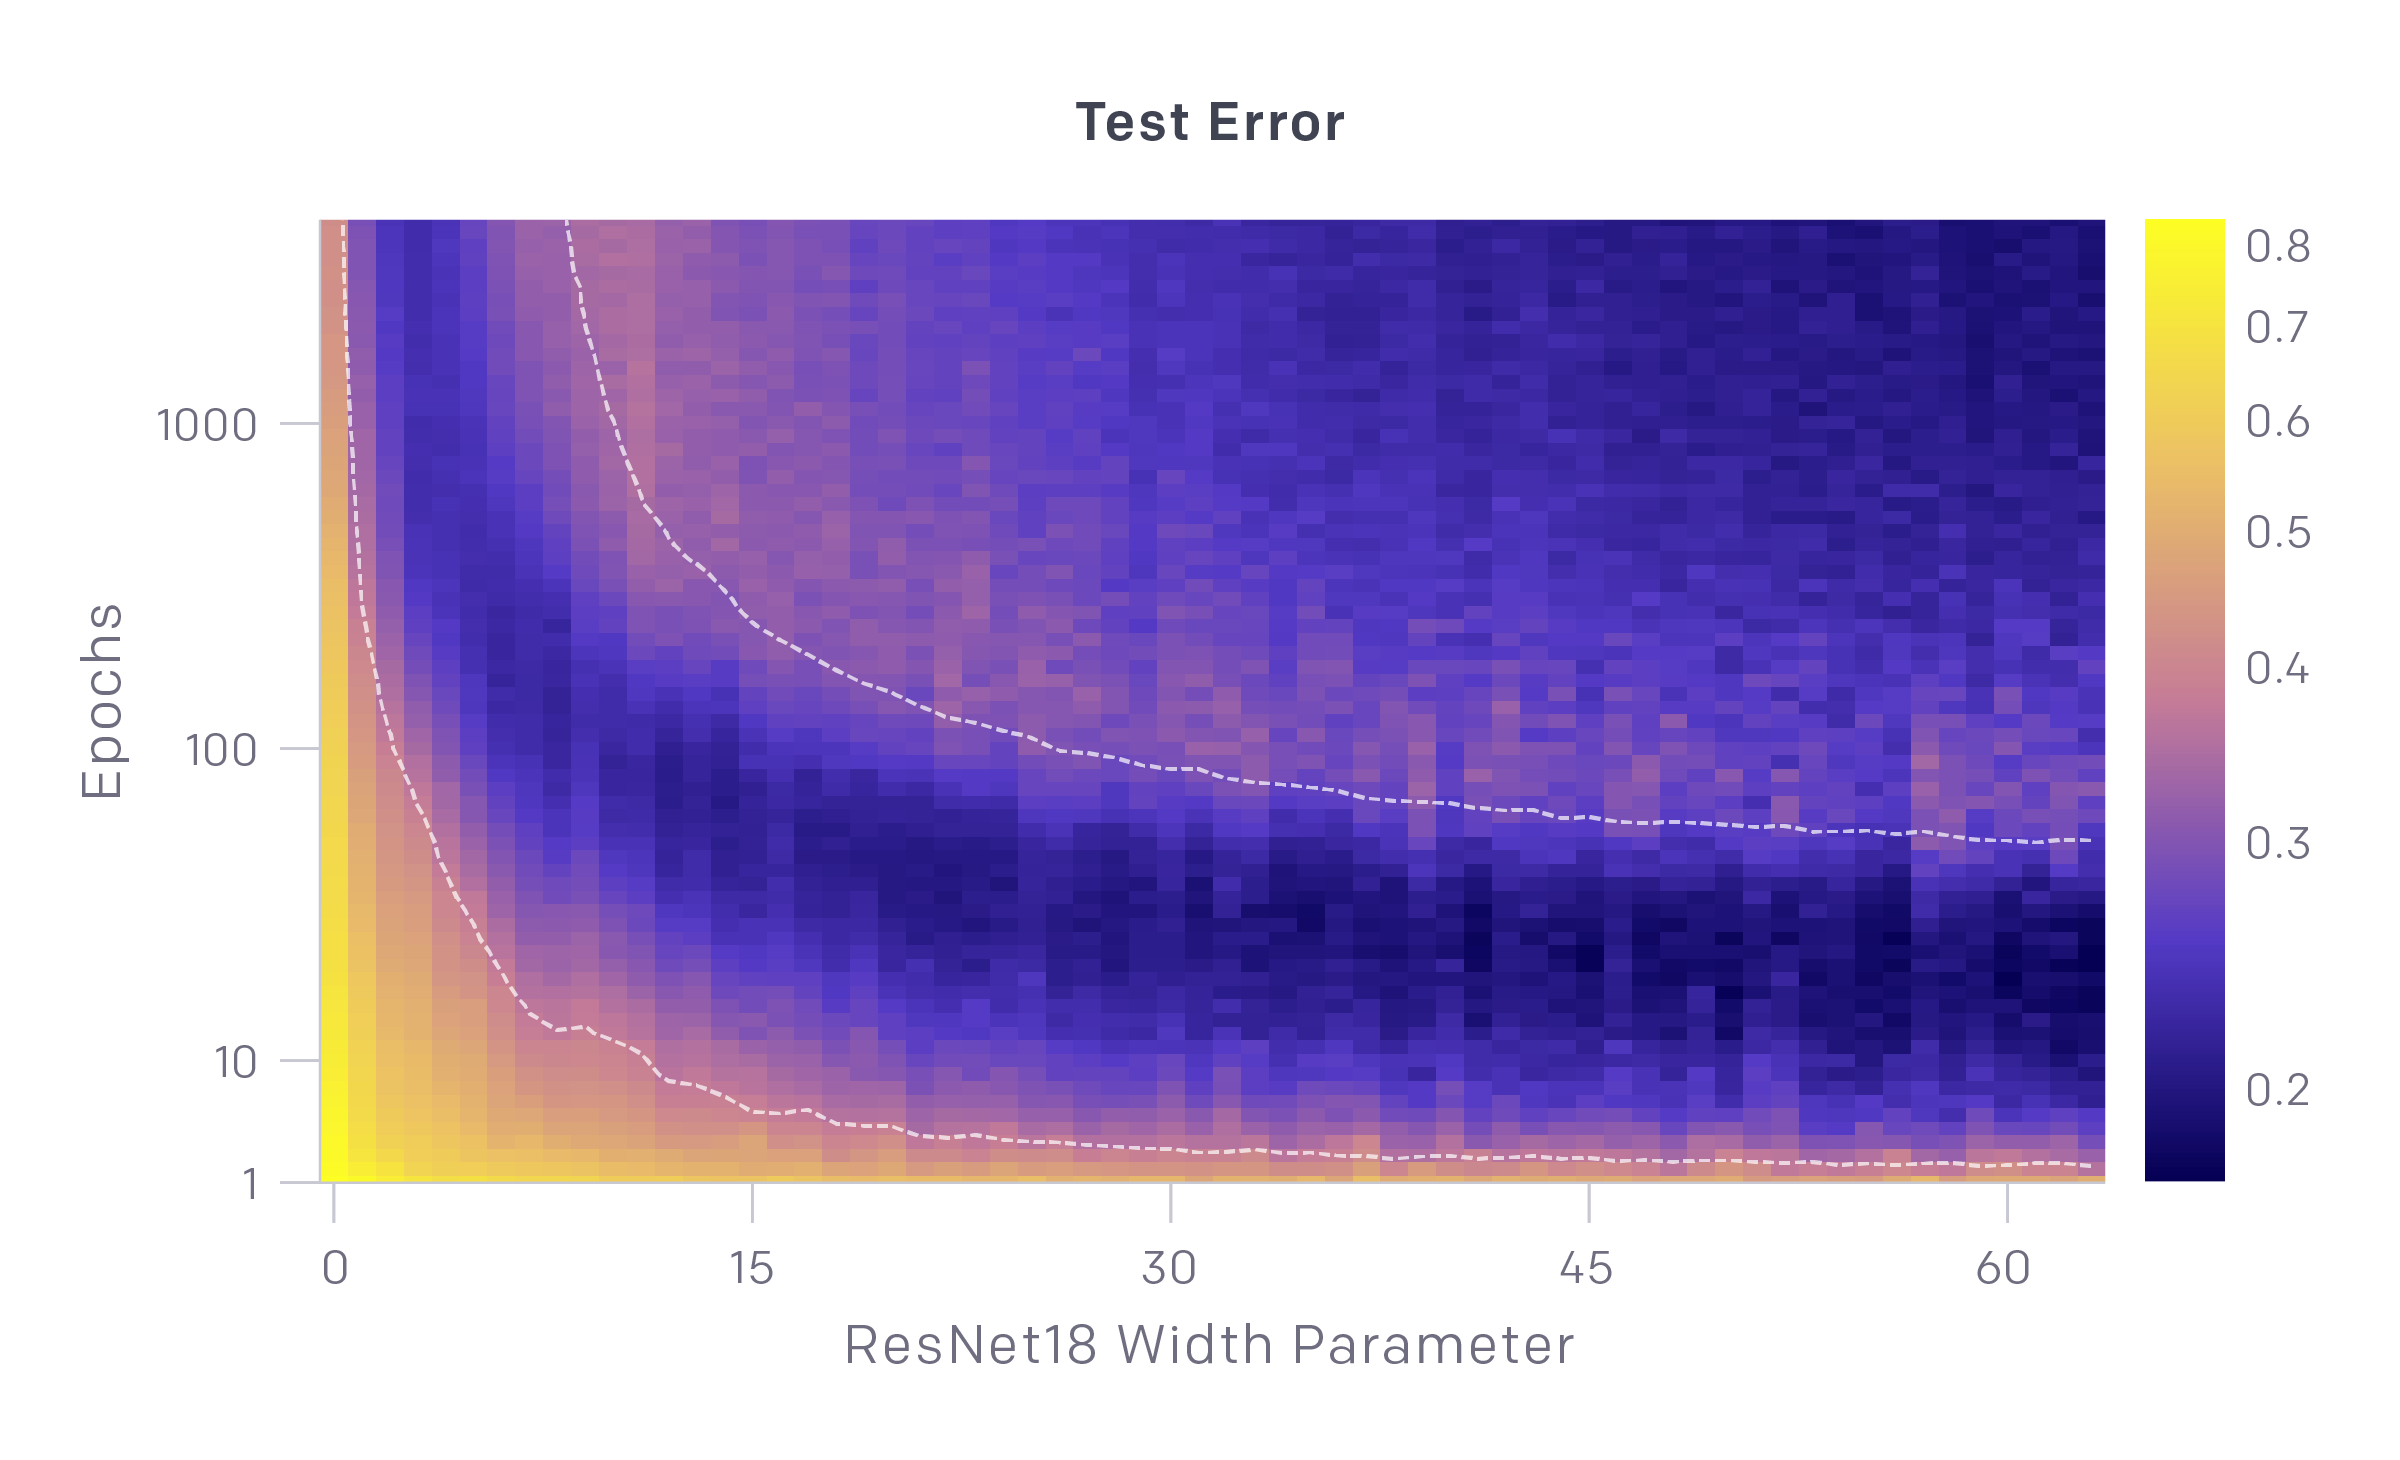
\includegraphics[scale=0.1]{double-descent/dd1.png}
\end{center}

\begin{enumerate}
    \item \points{3a}
\textbf{Plot Analysis.}
\begin{center}
    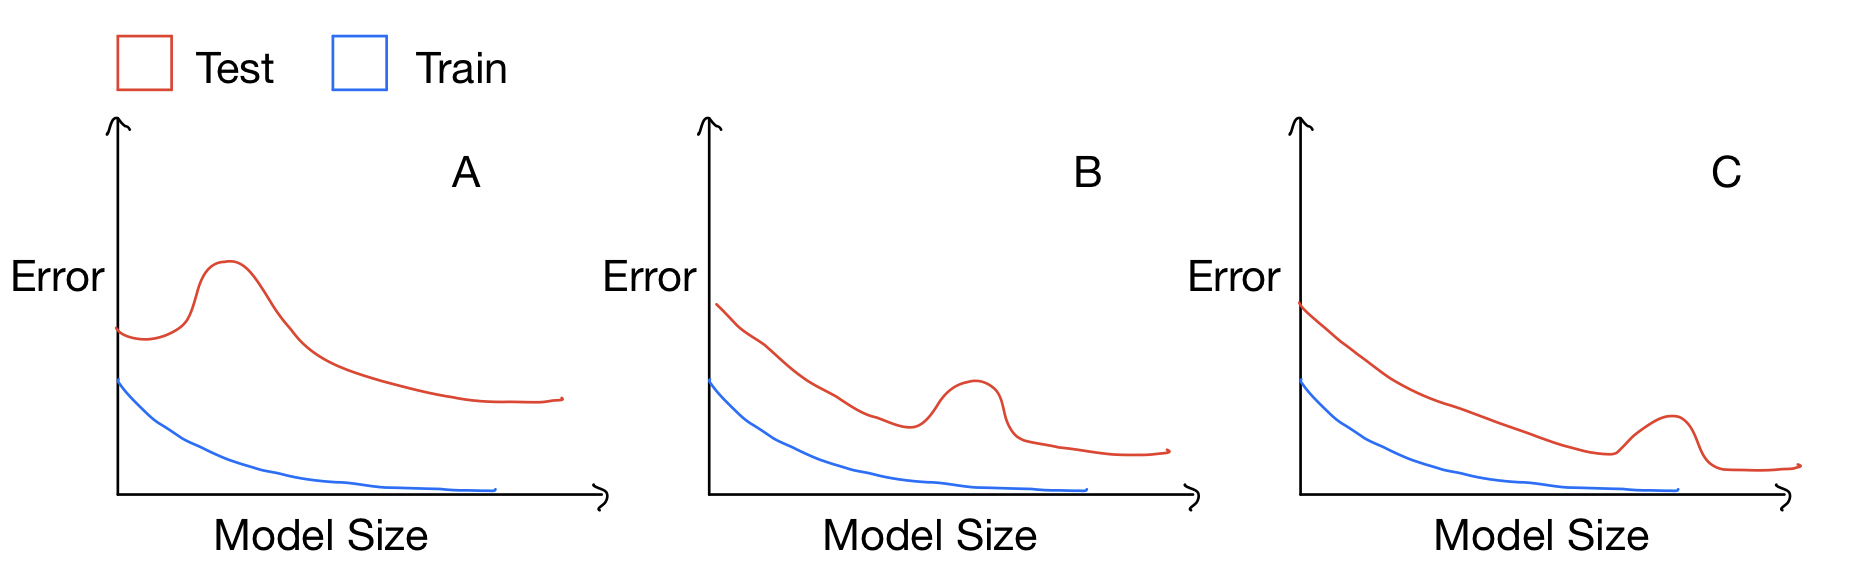
\includegraphics[scale=0.25]{double-descent/IMG_0633.jpg}
\end{center}
Which of the following plots of test/train accuracy would you most likely see when studying double descent? Select one option below.

\begin{enumerate}[label=(\alph*)]
    \item Plot A
    \item Plot B
    \item Plot C
\end{enumerate} 

    \begin{answer}
% ### START CODE HERE###
% ### END CODE HERE###
\end{answer}


    \item\points{3b}
\textbf{Explaining Double Descent.}
Which of the following reasons explain why we see double descent? Select all that apply.

\begin{enumerate}[label=(\alph*)]
    \item The weights which allow an under-parameterized model to (over)fit the training data are unlikely to generalize to unseen data.
    \item Under-parameterized models are unable to fit the training data, hence they perform worse than over parameterized models.
    \item When models are overparameterized the randomness of SGD sometimes ends up training models which generalize well.
    \item In the over-parameterized regime the implicit bias of SGD results in finding solutions that generalize well to unseen data.
\end{enumerate} 

    \begin{answer}
% ### START CODE HERE###
% ### END CODE HERE###
\end{answer}


    \item\points{3c}
\textbf{Training Data.}
Which of the following is the most likely reason for the regime where having more training data hurt the performance of the model? Select one option below.

\begin{enumerate}[label=(\alph*)]
    \item The additional data may not have the same distribution as the original data, making it harder for the model to find patterns in the data.
    \item It takes longer to train on more data, meaning there likely weren’t as many iterations for tuning the hyperparameters.
    \item The size and location of the double descent peaks are unpredictable and not yet understood. This is one possible way they can manifest in the training/testing process.
    \item Since the critical regime for training on more data is shifted to the right, the double descent peaks don’t line up. This results in the behavior we see.
\end{enumerate} 

    \begin{answer}
% ### START CODE HERE###
% ### END CODE HERE###
\end{answer}


\end{enumerate}
